% This part is to be filled by Lars

\begin{frame}{Na\"ive Approach}
  \begin{columns}
    \begin{column}{0.5\textwidth}
      \begin{itemize}
        \item Test out all possible paths
        \item Keep the shortest one
        \item Using Fast iterative enumeration algorithm \cite{nayuki_next_nodate}
        \item First Optimization: Fixate the first element!
        \item Complexity: $\Theta(n!)$
      \end{itemize}
    \end{column}
    \pause
    \begin{column}{0.5\textwidth}
      \begin{figure}
      \footnotesize\inputminted[xleftmargin=1em,fontsize=\tiny,linenos]{rust}{./assets/02_first_impl.rs}
      \end{figure}
    \end{column}
  \end{columns}
\end{frame}

\begin{frame}{Cache Prefix Sums}
  \begin{columns}
    \begin{column}{0.5\textwidth}
      \begin{itemize}
        \item After every path, we compute the tour
        \item Reuse partial computations
        \item While enumerating, keep prefix as long as possible
          \begin{itemize}
            \item \textbf{Recursive enumeration!}
          \end{itemize}
      \end{itemize}
    \end{column}
    \pause
    \begin{column}{0.5\textwidth}
      \begin{figure}
      \footnotesize\inputminted[xleftmargin=1em,fontsize=\small,linenos]{python}{./assets/02_recenum.py}
      \end{figure}
    \end{column}
  \end{columns}
  \pause
  \begin{center}
    {\Large But do we \textit{actually} have to look at every solution?}
  \end{center}
\end{frame}

\begin{frame}{Pruning}
  \vspace*{-0.5cm}
  \begin{columns}
    \begin{column}{0.5\textwidth}
      \begin{block}{V1: Stop what doesn't work!}
        \begin{itemize}
          \item Use the partial sum
          \item Lower bound: Previous best
          \item {\small\texttt{if (partial\_sum <= prev\_best) rec\_enum(...)}}
        \end{itemize}
      \end{block}
      \pause
      \begin{block}{V2: Nearest Neighbour (NN)}
        \begin{itemize}
          \item prune if \texttt{(partial\_sum + lower\_bound)} of remaining vertices
          \item Lower bound:
            \begin{itemize}
              \item Connect every vertex to the nearest one!
            \end{itemize}
        \end{itemize}
      \end{block}
    \end{column}
    \pause
    \begin{column}{0.5\textwidth}
      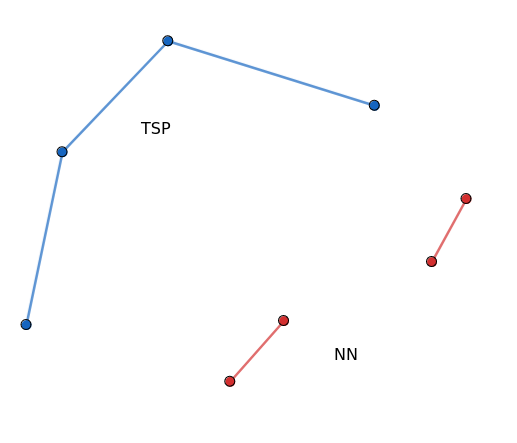
\includegraphics[width=\textwidth]{./assets/nn.png}
    \end{column}
  \end{columns}
\end{frame}

\begin{frame}{Pruning (cont.)}
  \vspace*{-0.5cm}
  \begin{columns}
    \begin{column}{0.5\textwidth}
      \begin{block}{V3: Minimal Spanning Tree (MST)}
        \begin{itemize}
          \item Same idea
          \item Use Minimal Spanning Tree of remaining vertices
          \item $NN < MST < TSP$
        \end{itemize}
      \end{block}
      \pause
      \begin{block}{V4: Caching}
        \begin{itemize}
          \item Cache the MST in a HashMap
          \item Using a non-cryptographic HashMap
        \end{itemize}
      \end{block}
    \end{column}
    \pause
    \begin{column}{0.5\textwidth}
      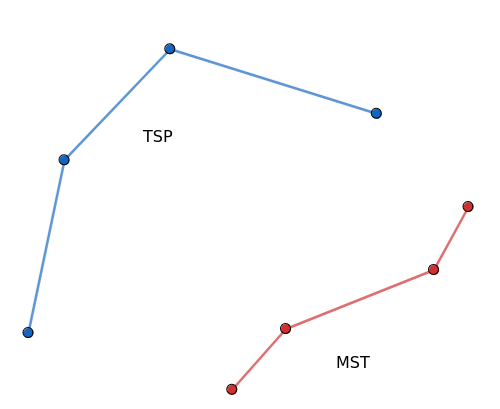
\includegraphics[width=\textwidth]{./assets/mst.png}
    \end{column}
  \end{columns}
\end{frame}

\begin{frame}{Benchmarking Results}
  \vspace{-0.25cm}
  \begin{figure}
    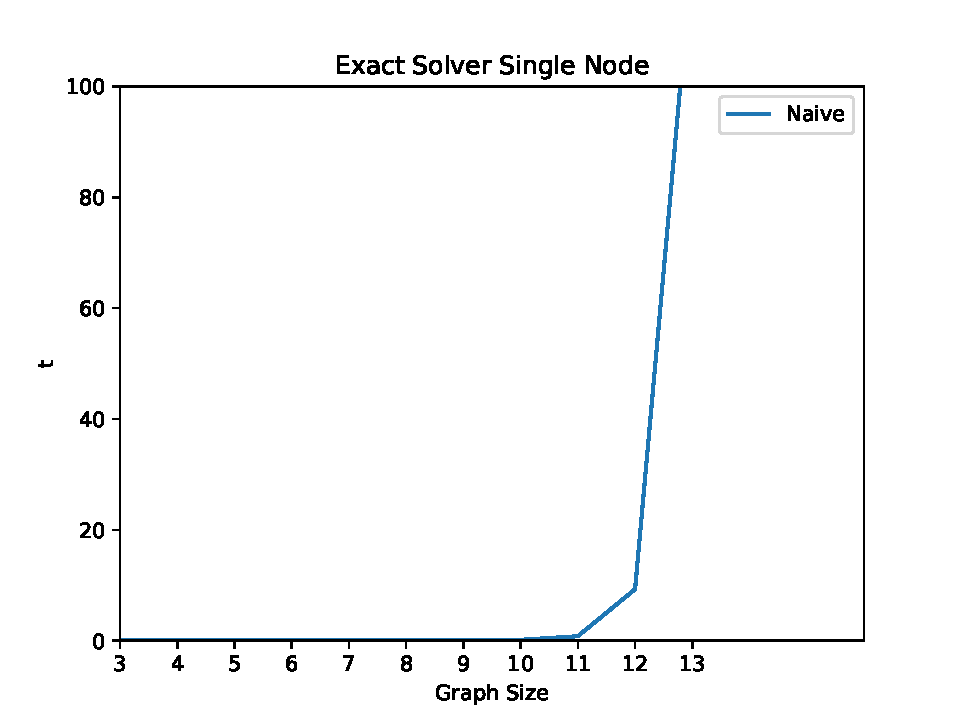
\includegraphics[width=\linewidth,height=.9\textheight,keepaspectratio]{./assets/v0.pdf}
  \end{figure}
\end{frame}
\begin{frame}{Benchmarking Results}
  \vspace{-0.25cm}
  \begin{figure}
    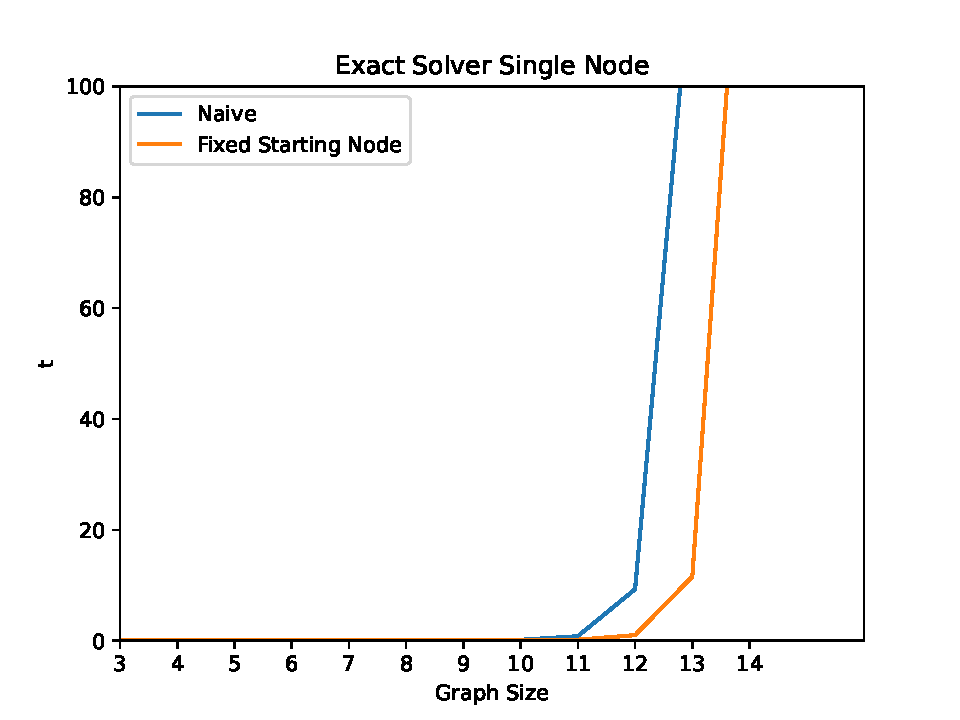
\includegraphics[width=\linewidth,height=.9\textheight,keepaspectratio]{./assets/v1.pdf}
  \end{figure}
\end{frame}
\begin{frame}{Benchmarking Results}
  \vspace{-0.25cm}
  \begin{figure}
    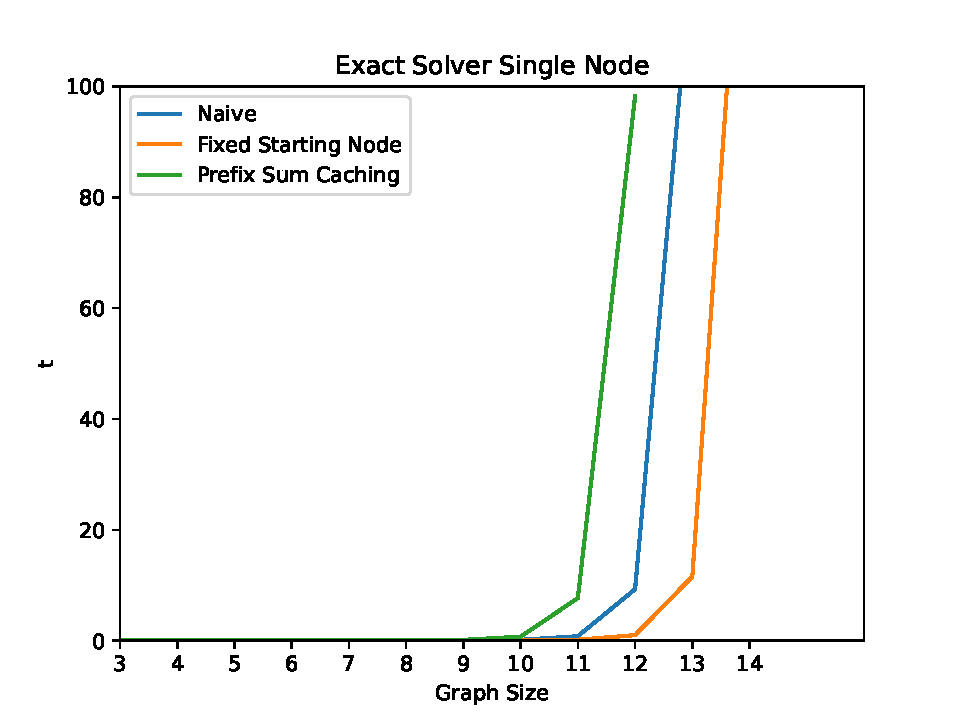
\includegraphics[width=\linewidth,height=.9\textheight,keepaspectratio]{./assets/v2.pdf}
  \end{figure}
\end{frame}
\begin{frame}{Benchmarking Results}
  \vspace{-0.25cm}
  \begin{figure}
    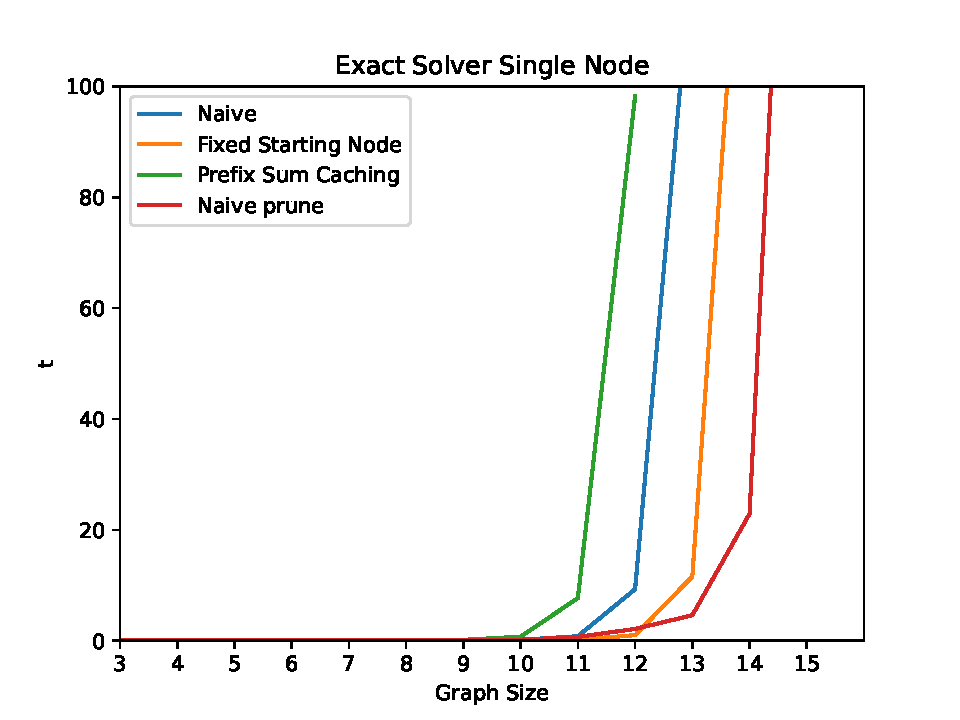
\includegraphics[width=\linewidth,height=.9\textheight,keepaspectratio]{./assets/v3.pdf}
  \end{figure}
\end{frame}
\begin{frame}{Benchmarking Results}
  \vspace{-0.25cm}
  \begin{figure}
    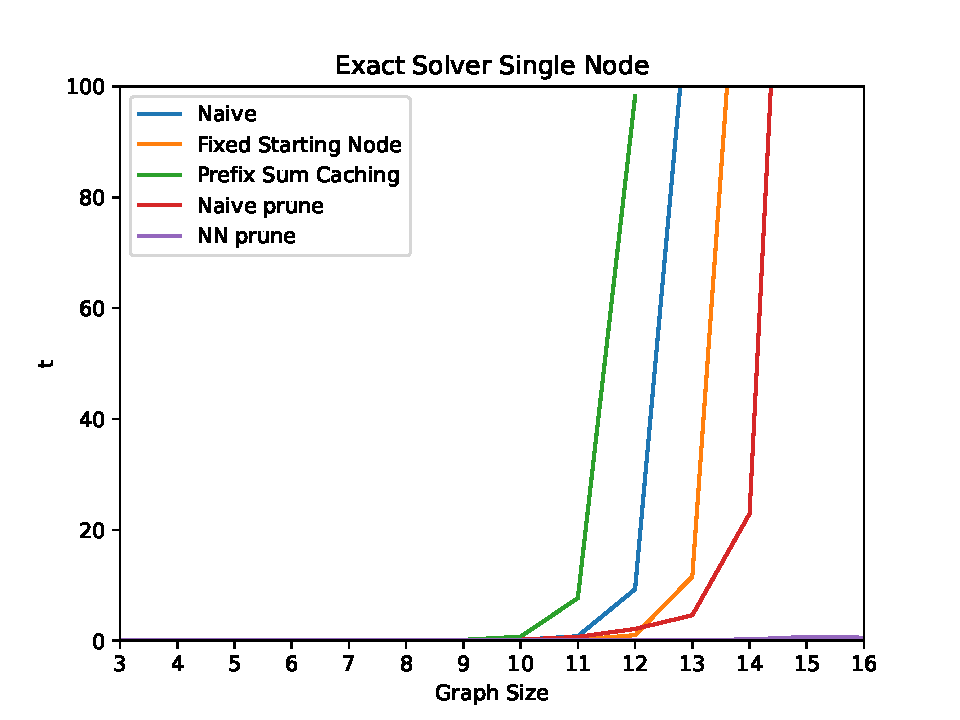
\includegraphics[width=\linewidth,height=.9\textheight,keepaspectratio]{./assets/v4.pdf}
  \end{figure}
\end{frame}
\begin{frame}{Benchmarking Results}
  \vspace{-0.25cm}
  \begin{figure}
    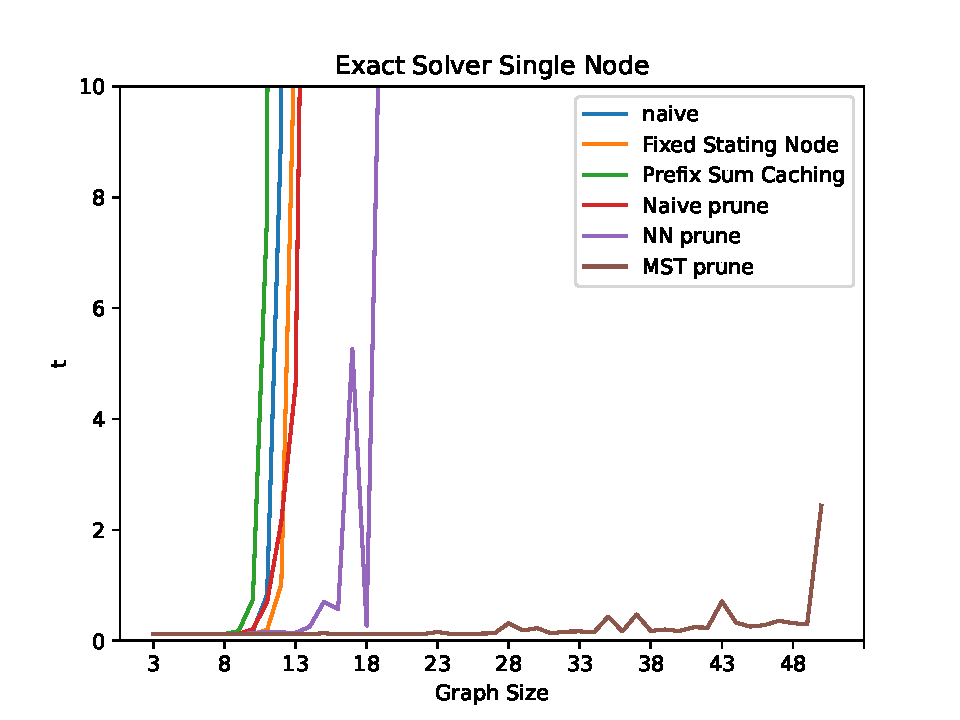
\includegraphics[width=\linewidth,height=.9\textheight,keepaspectratio]{./assets/v5.pdf}
  \end{figure}
\end{frame}
\begin{frame}{Benchmarking Results}
  \vspace{-0.25cm}
  \begin{figure}
    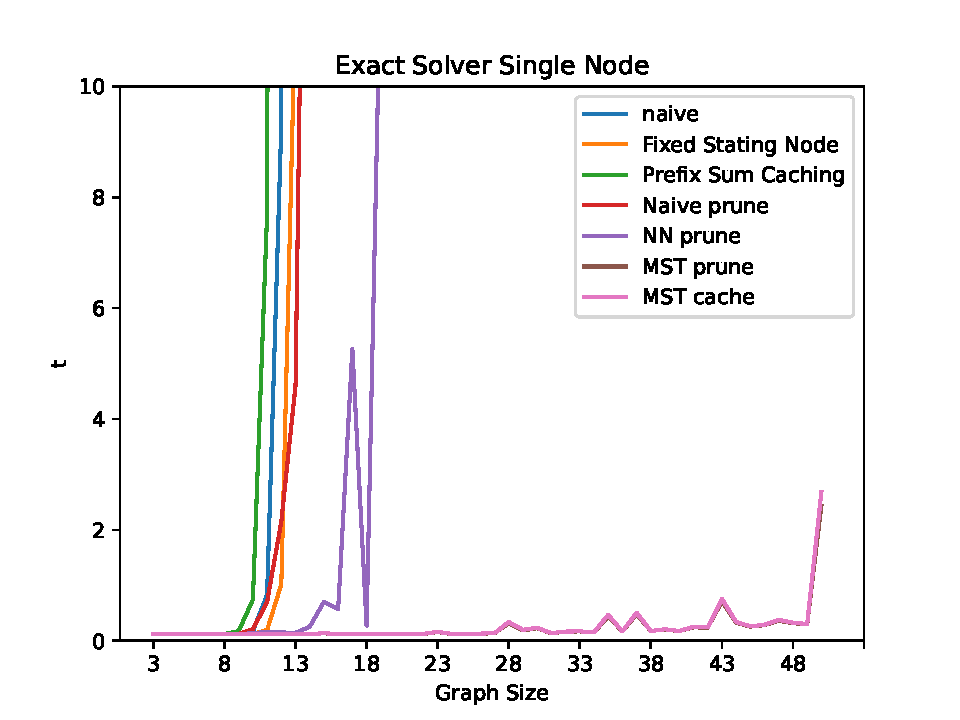
\includegraphics[width=\linewidth,height=.9\textheight,keepaspectratio]{./assets/v6.pdf}
  \end{figure}
\end{frame}

\begin{frame}{Threading}
  \begin{block}{Algorithm}
    \begin{enumerate}
        \pause
      \item Spawn $n$ threads
        \pause
      \item Divide the prefix space locally, $i$-th thread gets $i$-th chunk
        \pause
      \item Compute next prefix (with MST lower bound)
        \pause
      \item Update local optimum shared with all threads
        \pause
      \item \texttt{GOTO 3} until done with chunk
    \end{enumerate}
  \end{block}
\end{frame}
\begin{frame}{Benchmarking Results}
  \vspace{-0.25cm}
  \begin{figure}
    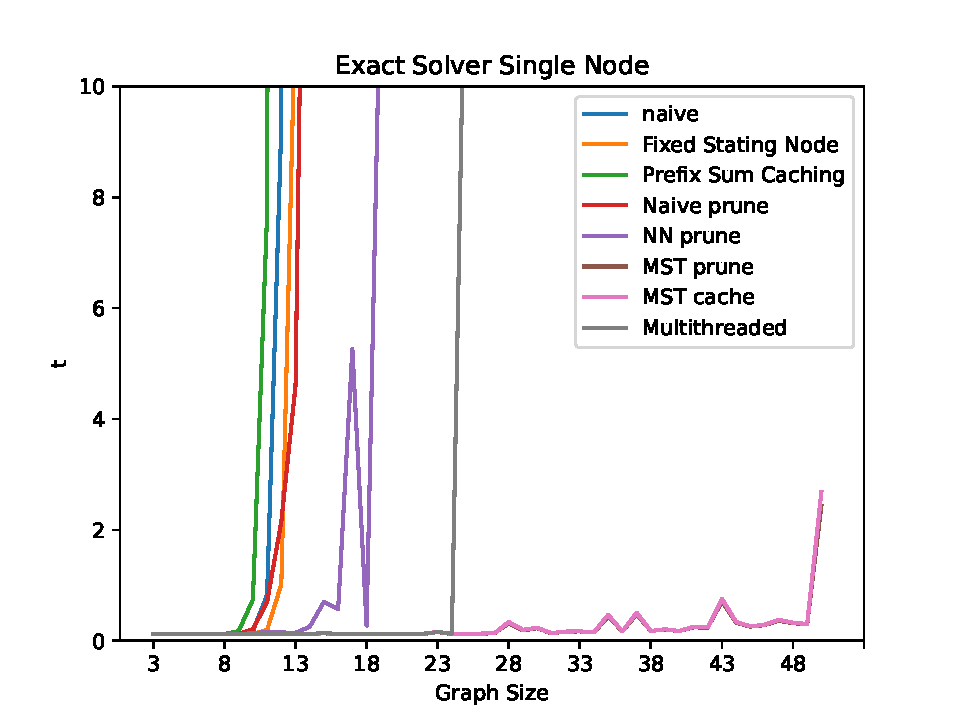
\includegraphics[width=\linewidth,height=.9\textheight,keepaspectratio]{./assets/v7.pdf}
  \end{figure}
\end{frame}

\begin{frame}{MPI}
  \begin{block}{Computation}
  \begin{itemize}
    \item One coordinator, $n-1$ worker
      \pause
    \item Prefix chunk division like threaded
      \pause
    \item After each prefix, the worker reports current best \textbf{cost} to coordinator
      \pause
    \item Coordinator answers with global best \textbf{cost}
      \begin{itemize}
        \item Tightest possible bound for pruning
      \end{itemize}
      \pause
    \item At the end, worker tells coordinator that its done and waits at barrier
      \pause
    \item After all are done, coordinator joins the barrier
  \end{itemize}
  \end{block}
\end{frame}

\begin{frame}{MPI (cont.)}
  \begin{block}{Joining the local optima}
  \begin{itemize}
      \pause
    \item After all are done, the coordinator broadcasts
      \begin{itemize}
        \item which rank won
        \item and the minimal cost
      \end{itemize}
      \pause
    \item That rank then broadcasts \textbf{the full path}
      \begin{itemize}
        \item This is an traffic efficiency optimization!
      \end{itemize}
  \end{itemize}
  \pause
  Now every process knows the best cost and path.
  \end{block}
\end{frame}

\begin{frame}{Benchmarks}
  \vspace{-0.25cm}
  \begin{figure}
    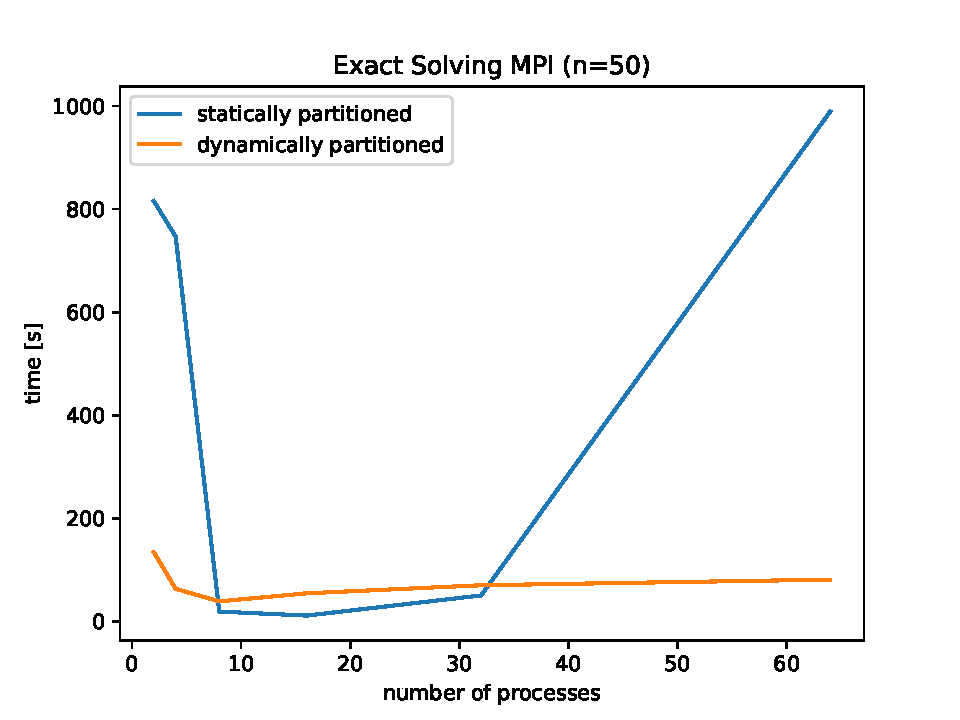
\includegraphics[width=\linewidth,height=.9\textheight,keepaspectratio]{./assets/exact-mpi.pdf}
  \end{figure}
\end{frame}
